\documentclass[12pt]{article}
\usepackage[utf8]{inputenc}
\usepackage[T1]{fontenc}
\usepackage{polski}
\usepackage{graphicx}
\usepackage{enumitem}
\usepackage{geometry}
\usepackage{booktabs}
\usepackage{hyperref}
\usepackage{pgfplots}
\pgfplotsset{compat=1.18}
\geometry{margin=2.5cm}

\title{Biometria -- Projekt 3: Uwierzytelnianie in-the-wild}
\author{
Marcel Masiukiewicz \\
Bartlomiej Ruszaj \\
Szymon Szafraniec \\
Marcin Tkocz
}
\date{Czerwiec 2026}

\begin{document}

\maketitle

\section{Dane autorow}

\begin{itemize}
    \item Marcel Masiukiewicz, nr indeksu: \textbf{TODO}, termin laboratorium: \textbf{TODO}
    \item Bartlomiej Ruszaj, nr indeksu: \textbf{TODO}, termin laboratorium: \textbf{TODO}
    \item Szymon Szafraniec, nr indeksu: \textbf{TODO}, termin laboratorium: \textbf{TODO}
    \item Marcin Tkocz, nr indeksu: \textbf{TODO}, termin laboratorium: \textbf{TODO}
\end{itemize}

\section{Cel projektu}

Celem projektu bylo rozszerzenie systemu uwierzytelniania biometrycznego tak, aby radzil sobie z probkami pobieranymi w warunkach \textit{in-the-wild}, czyli bez pelnej kontroli nad jakoscia danych wejsciowych. Zgodnie z trescia projektu P3 nalezalo wybrac co najmniej dwa utrudnienia i pokazac, ze probki trudne nie powoduja istotnego pogorszenia metryk wzgledem probek czystych.

W przypadku weryfikacji przyjeto wymaganie, ze wspolczynnik FRR dla probek trudnych nie powinien wzrosnac o wiecej niz 5 punktow procentowych wzgledem probek czystych, przy jednoczesnej minimalizacji FAR.

W raporcie opisano dwa wybrane problemy:

\begin{enumerate}
    \item Identyfikacja / weryfikacja twarzy na zdjeciach o niskiej rozdzielczosci lub niskiej jakosci, np. CCTV.
    \item Identyfikacja / weryfikacja glosu dla utrudnienia: \textbf{TODO: wpisac wybrane utrudnienie z P3, np. nagrania z duzym poziomem halasu / inny jezyk / dialog wielu osob / antispoofing}.
\end{enumerate}

\section{Zrodla i wykorzystane komponenty}

\begin{itemize}
    \item Tresc projektu P3: \texttt{P3.pdf}.
    \item ArcFace / InsightFace -- model rozpoznawania twarzy oparty o embeddingi twarzy i podobienstwo cosinusowe: \url{https://github.com/deepinsight/insightface}.
    \item MediaPipe Face Landmarker -- detekcja i punkty charakterystyczne twarzy: \url{https://developers.google.com/mediapipe}.
    \item CelebA -- zbior zdjec twarzy i identyfikatorow osob: \url{https://mmlab.ie.cuhk.edu.hk/projects/CelebA.html}.
    \item TinyFace -- inspiracja dla problemu bardzo malych twarzy / low-resolution face recognition: \url{https://qmul-tinyface.github.io/}.
    \item SpeechBrain ECAPA-TDNN -- ekstraktor embeddingow glosu: \url{https://speechbrain.github.io/}.
    \item Mozilla Common Voice -- zbior nagran mowy: \url{https://commonvoice.mozilla.org/}.
\end{itemize}

\section{Opis systemu}

System BioDesk jest aplikacja FastAPI z prostym interfejsem HTML/CSS/JavaScript. Obsluguje dwie modalnosci:

\begin{itemize}
    \item twarz -- ArcFace + MediaPipe Face Landmarker,
    \item glos -- ECAPA-TDNN + SpeechBrain + tor preprocessingu audio.
\end{itemize}

System udostepnia:

\begin{itemize}
    \item rejestracje uzytkownika,
    \item weryfikacje $1{:}1$ z podanym identyfikatorem,
    \item identyfikacje $1{:}N$ w calej bazie,
    \item panel eksperymentow i diagnostyki.
\end{itemize}

W bazie SQLite przechowywane sa embeddingi biometryczne, a nie surowe obrazy ani nagrania. Dla twarzy embedding ma wymiar 512, a dla glosu 192. Porownanie odbywa sie przez podobienstwo cosinusowe i prog decyzyjny.

\section{Problem 1: twarz o niskiej rozdzielczosci lub jakosci}

\subsection{Opis problemu}

Pierwszym utrudnieniem sa zdjecia twarzy o bardzo niskiej rozdzielczosci lub niskiej jakosci, np. pochodzace z kamer CCTV. W takim scenariuszu twarz moze zajmowac mala czesc kadru, byc rozmyta, zaszumiona, ciemna lub miec niski kontrast.

Problem jest istotny, poniewaz modele rozpoznawania twarzy, takie jak ArcFace, sa zwykle trenowane na relatywnie dobrze wykadrowanych i wyraznych obrazach. Gdy obraz zostanie silnie zdegradowany, embedding tej samej osoby moze odsunac sie od embeddingu referencyjnego, co zwieksza FRR.

\subsection{Metoda bazowa}

Metoda bazowa dla twarzy wykorzystuje nastepujacy tor:

\begin{center}
\texttt{obraz -> MediaPipe Face Landmarker -> alignment 112x112 -> ArcFace -> embedding -> cosine similarity}
\end{center}

Przy rejestracji uzytkownika system pobiera kilka klatek twarzy, liczy embedding dla kazdej z nich, usrednia embeddingi i ponownie normalizuje wynik. Przy weryfikacji pojedyncza probka jest porownywana z zapisanym profilem uzytkownika.

\subsection{Modyfikacje zwiekszajace odpornosc}

W ramach P3 dodano do systemu kilka mechanizmow zwiekszajacych odpornosc na low-res / CCTV:

\begin{itemize}
    \item modul oceny jakosci obrazu,
    \item rozroznienie probek \texttt{clean}, \texttt{low\_quality} oraz \texttt{reject},
    \item preprocessing dla probek low-quality,
    \item raportowanie ostrzezen jakosciowych w API,
    \item panel jakosci obrazu w GUI,
    \item eksperyment low-res uruchamiany z GUI,
    \item symulacja slabej jakosci w widoku autoryzacji.
\end{itemize}

\subsubsection{Ocena jakosci obrazu}

Dodany modul \texttt{face\_auth/quality.py} ocenia:

\begin{itemize}
    \item rozmiar obrazu,
    \item rozmycie przez wariancje Laplacianu,
    \item srednia jasnosc,
    \item kontrast,
    \item powodzenie detekcji i wyrownania twarzy.
\end{itemize}

Na tej podstawie system zwraca decyzje jakosciowa:

\begin{itemize}
    \item \texttt{clean} -- probka dobrej jakosci,
    \item \texttt{low\_quality} -- probka slabsza, ale nadal uzywalna,
    \item \texttt{reject} -- probka zbyt slaba do bezpiecznej autoryzacji.
\end{itemize}

\subsubsection{Preprocessing low-res}

Dodany modul \texttt{face\_auth/low\_quality.py} przygotowuje warianty obrazu, np. po powiekszeniu, poprawie kontrastu, odszumieniu i lekkim wyostrzeniu. Wariant robust moze policzyc kilka embeddingow dla roznych wersji tej samej probki i usrednic je w przestrzeni embeddingow.

W praktyce eksperyment pokazal, ze dla lagodnego low-res \texttt{64x64} i \texttt{80x80} standardowa sciezka ArcFace dziala bardzo dobrze, a dodatkowy robust preprocessing nie daje istotnej przewagi. Dlatego glowna wartoscia dodanych mechanizmow jest kontrola jakosci i odrzucanie probek skrajnie zniszczonych.

\subsubsection{Polityka jakosci}

Po eksperymentach przyjeto nastepujaca polityke:

\begin{itemize}
    \item \texttt{64x64}, \texttt{80x80} -- akceptowalny low-res / CCTV,
    \item \texttt{8x8}, \texttt{12x12}, \texttt{16x16}, \texttt{24x24}, \texttt{32x32}, \texttt{48x48} -- probki odrzucane jakosciowo.
\end{itemize}

Uzasadnienie: przy ekstremalnych degradacjach informacja biometryczna jest zbyt silnie usunieta. Bezpieczniej jest poprosic uzytkownika o ponowne pobranie probki niz obnizac prog i ryzykowac wzrost FAR.

\section{Problem 2: glos -- TODO}

\subsection{Opis problemu}

\textbf{TODO: opisac drugie wybrane utrudnienie z P3 dla glosu.}

Przykladowe warianty z listy P3:

\begin{itemize}
    \item nagrania z duzym poziomem halasu,
    \item wypowiedzi w innym jezyku niz probki uzyte przy wdrazaniu,
    \item dialogi lub rozmowa grupy osob,
    \item detekcja deepfake / spoofing / liveness.
\end{itemize}

\subsection{Metoda bazowa dla glosu}

Uwierzytelnianie glosu opiera sie na architekturze ECAPA-TDNN. Wykorzystywany jest model bazowy SpeechBrain \texttt{speechbrain/spkrec-ecapa-voxceleb}, a warstwa embeddingowa zostala douczona na polskim podzbiorze Common Voice.

Tor przetwarzania:

\begin{center}
\texttt{audio -> resampling 16 kHz mono -> ECAPA-TDNN -> embedding 192D -> cosine similarity}
\end{center}

Przy rejestracji system wymaga co najmniej trzech nagran. Dla kazdego nagrania liczony jest embedding, a wynikowy profil uzytkownika powstaje przez usrednienie embeddingow i normalizacje $\ell_2$.

\subsection{Modyfikacje odpornosci dla glosu}

\textbf{TODO: wpisac konkretne modyfikacje wykonane dla wybranego problemu glosowego.}

Przykladowa struktura opisu:

\begin{itemize}
    \item preprocessing audio,
    \item filtrowanie / normalizacja / przycinanie probki,
    \item test-time augmentation przez wiele wycinkow czasowych,
    \item ewentualna augmentacja lub korekta probek trudnych,
    \item sposob raportowania bledu lub odrzucenia probki.
\end{itemize}

\section{Zbiory danych i podzial}

\subsection{Dane dla twarzy}

Dla modalnosci twarzy wykorzystano CelebA oraz lokalne cropy twarzy przygotowane do rozmiaru \texttt{112x112}. Dane podzielono na splity:

\begin{itemize}
    \item \texttt{train\_split.txt} -- dane treningowe,
    \item \texttt{valid\_split.txt} -- dane walidacyjne,
    \item \texttt{test\_split.txt} -- dane testowe.
\end{itemize}

Do eksperymentu P3 wykorzystano split testowy. W eksperymencie low-res:

\begin{itemize}
    \item liczba uzytkownikow: 100,
    \item liczba probek czystych: 1000,
    \item liczba probek trudnych: 5000,
    \item probki czyste: cropy \texttt{112x112},
    \item probki trudne: syntetyczne degradacje \texttt{64x64} i \texttt{80x80}, nastepnie powiekszane do wejscia modelu.
\end{itemize}

Skrajne degradacje \texttt{8x8-48x48} potraktowano jako probki do odrzucenia jakosciowego, a nie jako probki do automatycznej decyzji biometrycznej.

\subsection{Dane dla glosu}

\textbf{TODO: opisac zbior danych dla wybranego problemu glosowego.}

Pola do uzupelnienia:

\begin{itemize}
    \item nazwa zbioru,
    \item liczba mowcow,
    \item liczba probek na mowce,
    \item czas trwania nagran,
    \item format i czestotliwosc probkowania,
    \item podzial train / valid / test,
    \item ktory podzbior byl uzywany do treningu, walidacji, testu i rejestracji uzytkownikow.
\end{itemize}

\section{Procedura wdrozenia}

\subsection{Wdrozenie profili twarzy}

Przy starcie system moze automatycznie zasilic baze profilami twarzy ze splitu testowego CelebA. Dla kazdej osoby wybierana jest probka referencyjna, z ktorej liczony jest embedding ArcFace. Embedding zapisywany jest w bazie SQLite.

\subsection{Wdrozenie profili glosu}

\textbf{TODO: opisac procedure wdrozenia profili glosu dla wybranego zbioru.}

Przykladowo: system pobiera co najmniej trzy nagrania dla uzytkownika, liczy embeddingi ECAPA-TDNN, usrednia je i zapisuje jeden szablon glosowy w bazie SQLite.

\section{Procedura uwierzytelniania}

\subsection{Twarz}

Dla twarzy procedura wyglada nastepujaco:

\begin{enumerate}
    \item pobranie klatki z kamery lub pliku,
    \item detekcja i wyrownanie twarzy,
    \item ocena jakosci probki,
    \item wybor sciezki: standard, low-res lub odrzucenie jakosciowe,
    \item obliczenie embeddingu ArcFace,
    \item porownanie z profilem uzytkownika przez cosine similarity,
    \item decyzja na podstawie progu.
\end{enumerate}

\subsection{Glos}

\textbf{TODO: opisac procedure uwierzytelniania glosu dla wybranego problemu.}

\section{Procedura testowania}

\subsection{Test twarzy low-res / CCTV}

Eksperyment twarzy uruchamiany jest z panelu GUI. Backend wywoluje predefiniowany skrypt:

\begin{center}
\texttt{scripts/evaluate\_low\_res\_face.py}
\end{center}

Skrypt zapisuje wynik do:

\begin{center}
\texttt{data/system/experiments/low\_res\_face\_latest.json}
\end{center}

Eksperyment obejmuje:

\begin{itemize}
    \item 100 uzytkownikow,
    \item 1000 probek czystych,
    \item 5000 probek trudnych,
    \item pomiar FRR i FAR,
    \item porownanie wyniku clean vs low-res.
\end{itemize}

\subsection{Test glosu}

\textbf{TODO: opisac procedure testowania drugiego problemu.}

Nalezy podac:

\begin{itemize}
    \item liczbe probek czystych,
    \item liczbe probek trudnych,
    \item sposob generowania lub pozyskania probek trudnych,
    \item metryki,
    \item prog decyzyjny,
    \item porownanie do wynikow clean.
\end{itemize}

\section{Wyniki}

\subsection{Wyniki dla twarzy}

\begin{table}[ht]
    \centering
    \begin{tabular}{lrr}
        \toprule
        Zbior / metoda & FRR & FAR \\
        \midrule
        Clean & 4.40\% & 0.50\% \\
        Low-res standard & 4.36\% & -- \\
        Low-res robust & 4.52\% & 0.56\% \\
        \bottomrule
    \end{tabular}
    \caption{Wyniki eksperymentu low-res / CCTV dla probek \texttt{64x64} i \texttt{80x80}.}
    \label{tab:face_low_res_results}
\end{table}

Wzrost FRR dla low-res robust wzgledem clean:

\begin{center}
\textbf{0.12 p.p.}
\end{center}

Poniewaz $0.12$ p.p. jest mniejsze niz dopuszczalne $5$ p.p., system spelnia wymaganie P3 dla probek low-res uznanych za uzywalne.

\begin{figure}[ht]
    \centering
    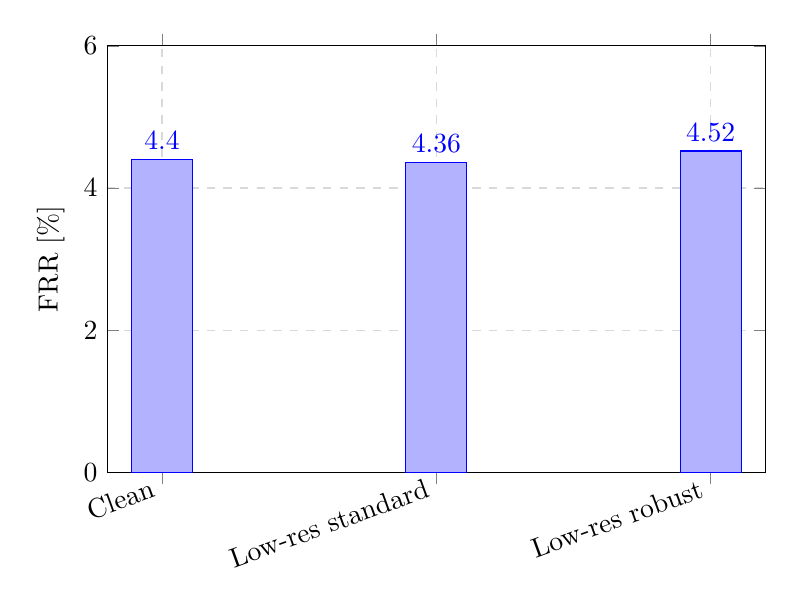
\begin{tikzpicture}
        \begin{axis}[
            ybar,
            width=0.82\textwidth,
            height=7cm,
            ymin=0,
            ymax=6,
            ylabel={FRR [\%]},
            symbolic x coords={Clean, Low-res standard, Low-res robust},
            xtick=data,
            x tick label style={rotate=20, anchor=east},
            nodes near coords,
            nodes near coords align={vertical},
            bar width=22pt,
            grid=major,
            major grid style={dashed, gray!30},
        ]
            \addplot coordinates {
                (Clean, 4.40)
                (Low-res standard, 4.36)
                (Low-res robust, 4.52)
            };
        \end{axis}
    \end{tikzpicture}
    \caption{Porownanie FRR dla probek czystych oraz low-res. Wyniki pokazuja, ze lagodne degradacje \texttt{64x64}/\texttt{80x80} nie powoduja istotnego wzrostu FRR.}
    \label{fig:face_low_res_frr}
\end{figure}

\begin{figure}[ht]
    \centering
    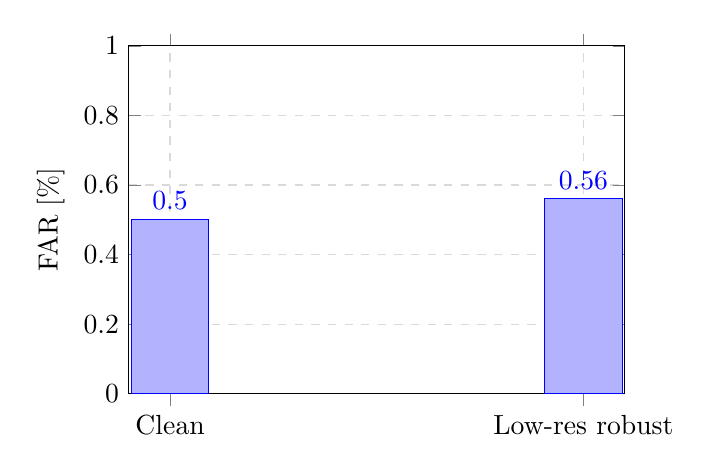
\begin{tikzpicture}
        \begin{axis}[
            ybar,
            width=0.65\textwidth,
            height=6cm,
            ymin=0,
            ymax=1,
            ylabel={FAR [\%]},
            symbolic x coords={Clean, Low-res robust},
            xtick=data,
            nodes near coords,
            nodes near coords align={vertical},
            bar width=28pt,
            grid=major,
            major grid style={dashed, gray!30},
        ]
            \addplot coordinates {
                (Clean, 0.50)
                (Low-res robust, 0.56)
            };
        \end{axis}
    \end{tikzpicture}
    \caption{Porownanie FAR dla probek czystych oraz wariantu low-res robust. FAR pozostaje zblizony do wyniku dla probek czystych.}
    \label{fig:face_low_res_far}
\end{figure}

\begin{figure}[ht]
    \centering
    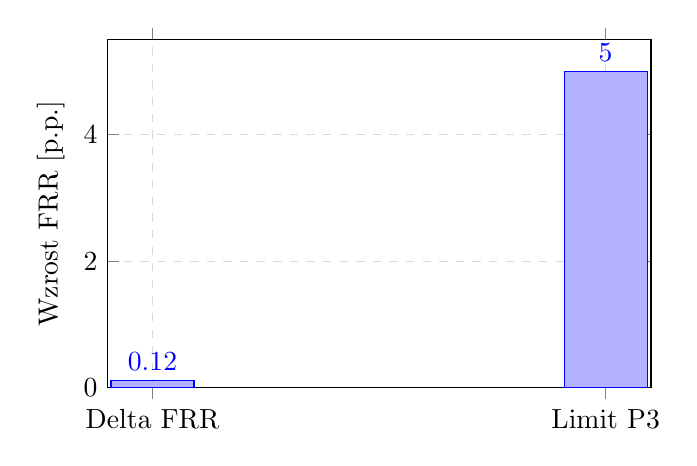
\begin{tikzpicture}
        \begin{axis}[
            ybar,
            width=0.7\textwidth,
            height=6cm,
            ymin=0,
            ymax=5.5,
            ylabel={Wzrost FRR [p.p.]},
            symbolic x coords={Delta FRR, Limit P3},
            xtick=data,
            nodes near coords,
            nodes near coords align={vertical},
            bar width=30pt,
            grid=major,
            major grid style={dashed, gray!30},
        ]
            \addplot coordinates {
                (Delta FRR, 0.12)
                (Limit P3, 5.00)
            };
        \end{axis}
    \end{tikzpicture}
    \caption{Porownanie wzrostu FRR z limitem P3. Uzyskany wzrost FRR wynosi $0.12$ p.p., czyli znacznie mniej niz dopuszczalne $5$ p.p.}
    \label{fig:face_low_res_p3_delta}
\end{figure}

\subsection{Wyniki dla glosu}

\textbf{TODO: uzupelnic tabela wynikow dla drugiego problemu.}

\begin{table}[ht]
    \centering
    \begin{tabular}{lrrr}
        \toprule
        Zbior / metoda & Metryka clean & Metryka trudne & Spadek / wzrost bledu \\
        \midrule
        TODO & TODO & TODO & TODO \\
        \bottomrule
    \end{tabular}
    \caption{Wyniki dla drugiego problemu glosowego.}
    \label{tab:voice_results}
\end{table}

\section{Porownanie z modelem bazowym i literatura}

\subsection{Twarz}

Model bazowy ArcFace jest silnym ekstraktorem embeddingow twarzy, ale jego skutecznosc zalezy od jakosci i rozdzielczosci wejscia. Wyniki pokazaly, ze przy ekstremalnych degradacjach \texttt{8x8-32x32} FRR rosnie bardzo silnie, natomiast dla lagodniejszych degradacji \texttt{64x64} i \texttt{80x80} system utrzymuje metryki blisko probek czystych.

\subsection{Glos}

\textbf{TODO: porownac wyniki glosu z modelem bazowym ECAPA-TDNN / SpeechBrain oraz wynikami z poprzednich eksperymentow.}

\section{Wnioski}

\subsection{Twarz}

Dla akceptowalnych probek low-res, czyli \texttt{64x64} i \texttt{80x80}, system spelnia wymaganie P3. FRR wzrosl tylko o $0.12$ punktu procentowego wzgledem probek czystych.

Jednoczesnie eksperymenty pokazaly, ze probki skrajnie zdegradowane \texttt{8x8-48x48} nie powinny byc przepuszczane przez system jako zwykle probki do autoryzacji. Bezpieczniejsze jest ich odrzucenie jakosciowe i poproszenie uzytkownika o ponowne pobranie obrazu.

\subsection{Glos}

\textbf{TODO: uzupelnic wnioski dla drugiego problemu.}

\section{Prezentacja dzialania systemu}

Podczas zajec laboratoryjnych nalezy pokazac:

\begin{itemize}
    \item rejestracje lub istniejace profile uzytkownikow,
    \item autoryzacje twarza dla obrazu czystego,
    \item autoryzacje twarza z symulacja \texttt{64x64} lub \texttt{80x80},
    \item odrzucenie jakosciowe dla symulacji \texttt{32x32} lub \texttt{48x48},
    \item uruchomienie eksperymentu low-res / CCTV z GUI,
    \item wynik JSON i podsumowanie P3,
    \item \textbf{TODO: demonstracje drugiego problemu glosowego}.
\end{itemize}

\end{document}
